\icode{E-MCH-MU-L2-261026-001}
（多选）
\(a\)、\(b\)两个物体做平抛运动的轨迹如图所示,设它们抛出的初速度分别为\(v_a\)、\(v_b\)、从抛出至碰到台上的时间分别为\(t_a\)、\(t_b\)，则\paren[]

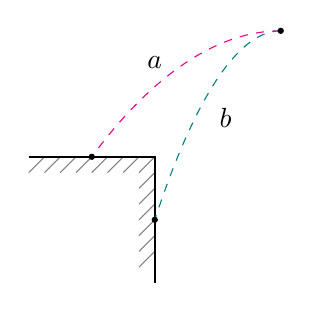
\begin{tikzpicture}
	\foreach \x in {-1.6,-1.4,...,0}
		\draw[gray] (\x,-.2)--++(.2,.2);
	\foreach \y in {-.4,-.6,...,-1.6}
		\draw[gray] (-.2,\y)--++(.2,.2);
	\draw[thick] (-1.6,0)--(0,0)--(0,-1.6);
	\draw[dashed,magenta] (1.6,1.6) parabola bend (1.6,1.6) (-.8,0);
	\draw[dashed,teal] (1.6,1.6) parabola bend (1.6,1.6) (0,-.8);
	\node at(0,1.2){ \(a\)};
	\node at(.9,.5){ \(b\)};
	\foreach \c in {(1.6,1.6),(-.8,0),(0,-.8)}
		\fill \c circle(.04);
\end{tikzpicture}
\begin{choices}
	\item \(v_a > v_b\)
	\item \(v_a < v_b\)
	\item \(t_a > t_b\)
	\item \(t_a < t_b\)
\end{choices}
\begin{answer}
	AD\qquad 提示：
\end{answer}